% ============================================================
%  Section 4: Input Representation
% ============================================================

\section{Input Representation}
\label{sec:input}

\bert{} does not operate on raw text but on a structured token sequence derived
through a combination of three additive embedding types.  This design allows a
single model to handle both single-sentence and sentence-pair inputs without any
architectural modification.

\subsection{Tokenisation}
\label{subsec:tokenisation}

Input text is first tokenised using \emph{WordPiece}~\cite{wu2016googles}, a
subword segmentation algorithm that decomposes rare or unseen words into frequent
sub-units drawn from a fixed vocabulary of 30,000 tokens.  For example, the word
\texttt{playing} may be split into \texttt{play} and \texttt{\#\#ing}, where the
prefix \texttt{\#\#} denotes a continuation piece.  This strategy balances
vocabulary coverage against embedding table size and reduces the out-of-vocabulary
rate to zero.

\begin{table}[H]
  \centering
  \caption{WordPiece tokenisation examples. Rare and out-of-vocabulary words are
           decomposed into frequent subword units.}
  \label{tab:tokenisation}
  \renewcommand{\arraystretch}{1.4}
  \begin{tabular}{ll}
    \toprule
    \textbf{Original Word} & \textbf{WordPiece Tokens} \\
    \midrule
    playing & [\texttt{play}, \texttt{\#\#ing}] \\
    unbelievable & [\texttt{un}, \texttt{\#\#believ}, \texttt{\#\#able}] \\
    transformer & [\texttt{transform}, \texttt{\#\#er}] \\
    \#\#ing & [\texttt{\#\#ing}] (subword only) \\
    \bottomrule
  \end{tabular}
\end{table}

\subsection{Embedding Components}
\label{subsec:embeddings}

Let $n$ denote the sequence length.  Each input position $i \in \{1, \ldots, n\}$
is associated with three embedding vectors, all of dimension $d$:

\begin{enumerate}
  \item \textbf{Token embeddings} $\mathbf{e}^{\text{tok}}_i$: a learned lookup
        table that maps each WordPiece token to a dense vector in $\R^d$.

  \item \textbf{Segment embeddings} $\mathbf{e}^{\text{seg}}_i$: one of two
        learned vectors ($\mathbf{E}_A$ or $\mathbf{E}_B$) indicating whether the
        token belongs to the first or second sentence in a sentence-pair input.
        For single-sentence inputs, all tokens receive $\mathbf{E}_A$.

  \item \textbf{Position embeddings} $\mathbf{e}^{\text{pos}}_i$: learned
        vectors for each absolute position $i \in \{0, \ldots, 511\}$, enabling
        the model to encode word order.  Note that these are \emph{learned} rather
        than the sinusoidal encodings used in the original Transformer.
\end{enumerate}

The final input representation for position $i$ is the element-wise sum:
\begin{equation}
  \mathbf{h}^{(0)}_i = \mathbf{e}^{\text{tok}}_i
    + \mathbf{e}^{\text{seg}}_i
    + \mathbf{e}^{\text{pos}}_i,
  \label{eq:embedding}
\end{equation}
and the resulting matrix $\mathbf{H}^{(0)} \in \R^{n \times d}$ is passed as
input to the first encoder layer.

\begin{figure}[H]
  \centering
  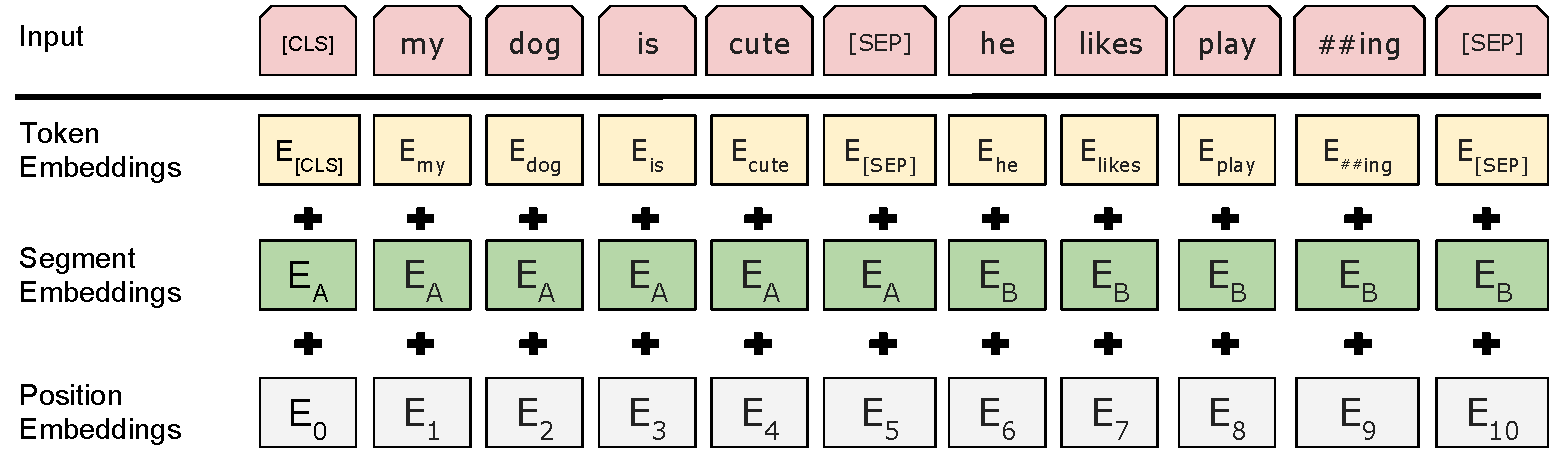
\includegraphics[width=0.90\textwidth]{figures/bert_input.pdf}
  \caption{\bert{} input representation for a sentence pair.  Each token embedding
           is summed with the corresponding segment embedding and position embedding.
           The special \cls{} token is prepended and \sep{} tokens delimit sentences.}
  \label{fig:bert_input}
\end{figure}

\subsection{Special Tokens}
\label{subsec:special_tokens}

\bert{} introduces two special tokens that carry structural significance:

\begin{itemize}
  \item \cls{} (\emph{classification token}): prepended to every input sequence.
        After passing through all $L$ encoder layers, the final hidden state
        corresponding to \cls{} aggregates a sentence-level (or sentence-pair-level)
        representation and is used as input to classification heads during
        fine-tuning.

  \item \sep{} (\emph{separator token}): inserted at the end of each sentence in a
        pair to provide an explicit boundary signal.  For single-sentence inputs, a
        single \sep{} is appended at the end.
\end{itemize}

\begin{remark}
  The maximum input length supported by BERT is 512 tokens (determined by the
  range of its learned position embeddings).  For documents exceeding this limit,
  truncation or sliding-window strategies must be employed.
\end{remark}
